\input{../../../.preambles/02-lab_work}
\newgeometry{top=1.5cm, bottom=1.5cm, left=1cm, right=1cm}
\begin{document}
    \begin{table}[h!]
        \center
        \begin{tabular}{|C{.5}|C{.2}|C{.25}|}
            \hline
            \multicolumn{1}{|c|}{\multirow{4}{*}{Лабораторная работа № 5}} &
            Студент, группа & {{ student }}, Ф-369 \\ \cline{2-3}
            & Дата выполнения & 02.03.2013 \\ \cline{2-3}
            & Подпись &  \\ \cline{2-3}
            Интегральные логические элементы & Дата отчёта & \\ \cline{2-3}
            & Оценка &  \\ \cline{2-3}
            & Подпись &  \\ \hline
        \end{tabular}
    \end{table}

    \emph{Цель работы:} научиться измерять основные параметры, снимать
    характеристики интегральных логических (цифровых) элементов в различных
    режимах.

    \begin{figure}[h!]
        \center
        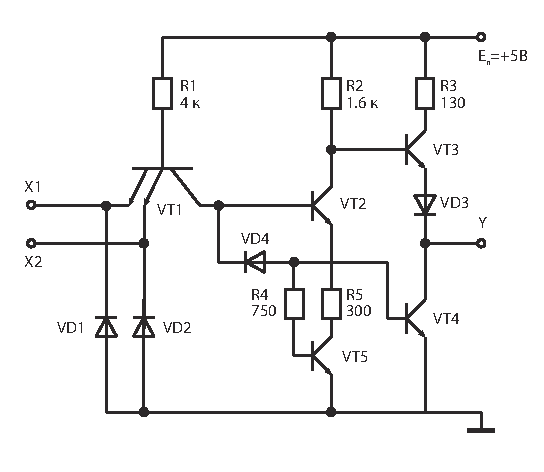
\includegraphics[width=.4\textwidth]{scheme}
        \caption{Принципиальная схема ЛЭ}
    \end{figure}

    \subsection{Уровни выходных напряжений ЛЭ. Нагрузочные характеристики
    \( U_\emph{вых} = f(I_H) \)}

    \begin{figure}[h!]
        \center
        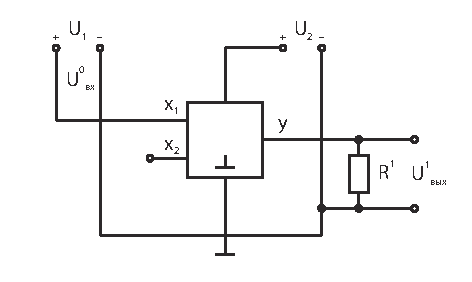
\includegraphics[width=.47\textwidth]{5-4-2_01} \hfill
        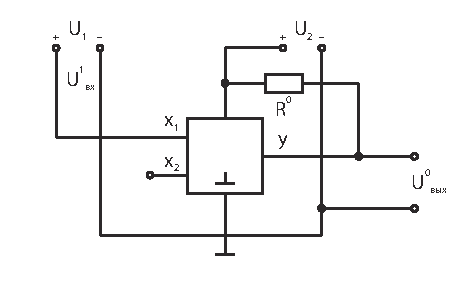
\includegraphics[width=.47\textwidth]{5-4-2_02}
        \parbox{.47\textwidth}{\caption{Схема для измерения
        \( {U^1}_\emph{вых} \)}} \hfill
        \parbox{.47\textwidth}{\caption{Схема для измерения
        \( {U^0}_\emph{вых} \)}}
    \end{figure}

    \begin{table}[h!]
        \center
        \caption{Результаты измерений и расчетов}
        \begin{tabular}{|*{2}{C{.1}|}*{6}{C{.07}|}} \hline
            & \multirow{2}{*}{Режим Х.Х.} & \multicolumn{3}{c|}{\( R^1 \),~кОм}
            & \multicolumn{3}{c|}{\( R^0 \),~кОм} \\ \cline{3-8}
            & & 22,0 & 10,0 & 6,8 & 2,2 & 1,5 & 1 \\ \hline
            \( {U^1}_\emph{вых} \),~В & 3,92 & 3,42 & 3,36 & 3,28
            & --- & --- & --- \\ \hline
            \( {U^0}_\emph{вых} \),~В & 4,92 & --- & --- & ---
            & 4,84 & 4,80 & 4,74 \\ \hline
            \( I_H \),~мА & 0 & 0,16 & 0,34 & 0,48
            & 2,20 & 3,20 & 4,74 \\ \hline
        \end{tabular}
    \end{table}

    \begin{figure}[h!]
        \center
        \includegraphics[width=.47\textwidth]{5-4-2_u0} \hfill
        \includegraphics[width=.47\textwidth]{5-4-2_u1}
        \parbox{.47\textwidth}{\caption{Зависимость тока нагрузки от напряжения
        \( {U^0}_\emph{вых} \)}} \hfill
        \parbox{.47\textwidth}{\caption{Зависимость тока нагрузки от напряжения
        \( {U^1}_\emph{вых} \)}}
    \end{figure}

    Ток нагрузки при \( {U^0}_\emph{вых} = 0,4 \)~В: \( I_{H_0} = 113,25 \)~мА.
    Ток нагрузки при \( {U^1}_\emph{вых} = 2,4 \)~В: \( I_{H_1} = 2,53\)~мА.

    \pagebreak

    \subsection{Входные токи ЛЭ}

    \begin{figure}[h!]
        \center
        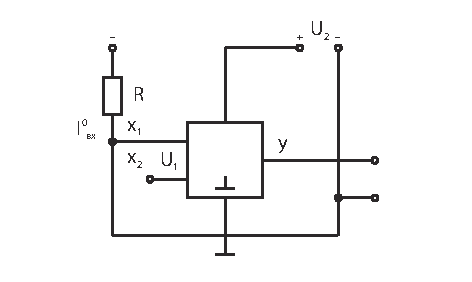
\includegraphics[width=.47\textwidth]{5-4-3_01} \hfill
        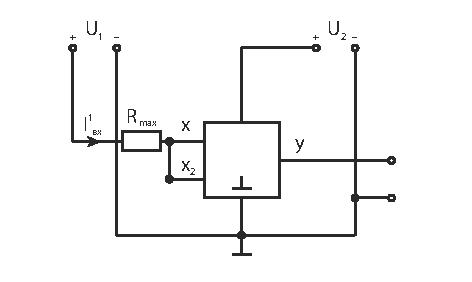
\includegraphics[width=.47\textwidth]{5-4-3_02}
        \parbox{.47\textwidth}{\caption{Схема для измерения
        \( {I^0}_\emph{вх} \)}} \hfill
        \parbox{.47\textwidth}{\caption{Схема для измерения
        \( {I^1}_\emph{вх} \)}}
    \end{figure}

    \begin{table}[h!]
        \center
        \caption{Результаты измерений и расчетов}
        \begin{tabular}{|C{.1}|C{.1}|C{.1}|C{.05}|C{.05}|C{.1}|C{.1}|} \hline
            \multicolumn{2}{|c|}{\( R \),~кОм} & \multicolumn{3}{c|}{\( U \),~В}
            & \multicolumn{2}{c|}{\( I \),~мА} \\ \hline
            \( R_{min} \) & \( R_{max} \) & \( U_0 \) & \( U_1^\emph{2В} \) &
            \( U_1^\emph{5В} \) & \( {I^0}_\emph{вх} \) & \( {I^1}_\emph{вх} \)
            \\ \hline
            1 & 100 & \( 13 \cdot 10^{-3} \) & 1,9 & 4,7 &
            &  \\ \hline
        \end{tabular}
    \end{table}
\end{document}
